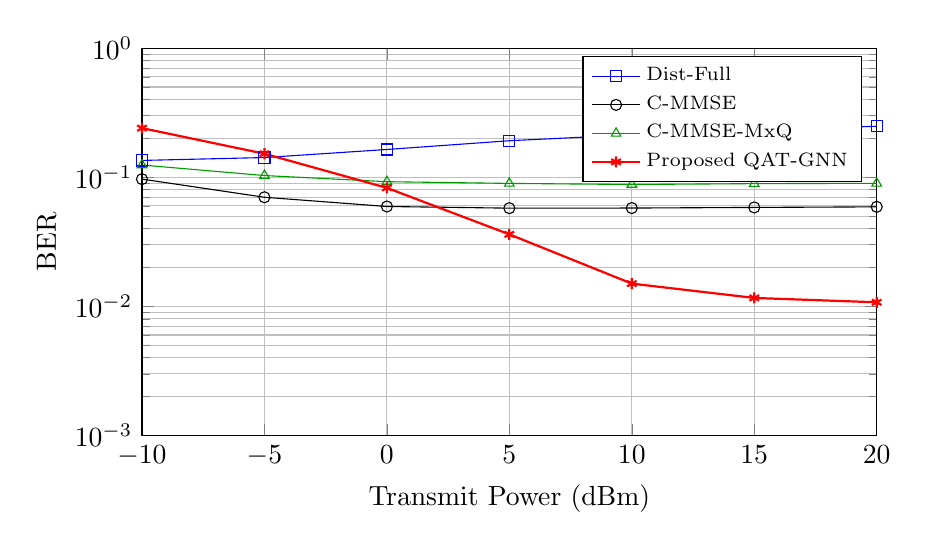
\begin{tikzpicture}
\begin{semilogyaxis}[
    width=0.9\linewidth,
    height=6.5cm,
    xlabel={Transmit Power (dBm)},
    ylabel={BER},
    xmin=-10, xmax=20,
    ymin=1e-3, ymax=1,
    grid=both,
    legend style={at={(0.98,0.98)},anchor=north east,font=\scriptsize},
    legend cell align={left}
]
\addplot[color=blue,mark=square] coordinates {
(-10, 0.13500) (-5, 0.14213) (0, 0.16412) (5, 0.19187) (10, 0.21325) (15, 0.23237) (20, 0.24825)
};
\addlegendentry{Dist-Full}

\addplot[color=black,mark=o] coordinates {
(-10, 0.09675) (-5, 0.07000) (0, 0.05937) (5, 0.05763) (10, 0.05775) (15, 0.05837) (20, 0.05900)
};
\addlegendentry{C-MMSE}

\addplot[color=green!60!black,mark=triangle] coordinates {
(-10, 0.12437) (-5, 0.10312) (0, 0.09238) (5, 0.08962) (10, 0.08788) (15, 0.08925) (20, 0.08975)
};
\addlegendentry{C-MMSE-MxQ}

\addplot[color=red,mark=asterisk,thick] coordinates {
(-10, 0.24025) (-5, 0.15213) (0, 0.08275) (5, 0.03612) (10, 0.01500) (15, 0.01162) (20, 0.01075)
};
\addlegendentry{Proposed QAT-GNN}
\end{semilogyaxis}
\end{tikzpicture}